\documentclass[11pt]{article}
\usepackage[margin=0.66in]{geometry}
\usepackage{booktabs,enumitem,fancyhdr,graphicx,tabularx,titlesec}
\usepackage[table]{xcolor}
\usepackage[hidelinks]{hyperref}
\graphicspath{{docs/lessons/assets/}{../assets/}}
\hypersetup{pdftitle={ADK Lesson 043: Copied Inertial Observations},
 pdfauthor={Kevin Shanahan},
 pdfsubject={Synthetic six-axis provenance, freshness, and diagnostic replay},
 pdflang={en-US}}
\pagestyle{fancy}\fancyhf{}
\lhead{\textsc{ADK Lesson 043}}\rhead{Copied Inertial Observations}
\cfoot{\thepage}\setlength{\headheight}{14pt}
\setlength{\parindent}{0pt}\setlength{\parskip}{4pt}
\setlist{nosep,leftmargin=1.45em}
\titleformat{\section}{\Large\bfseries}{\thesection}{0.5em}{}
\newcommand{\lessonbox}[1]{\begin{center}\fbox{\parbox{0.92\linewidth}{#1}}\end{center}}
\newcommand{\blankline}{\rule{0.9in}{0.4pt}}

\begin{document}
\begin{center}
 {\Huge\bfseries Copied Inertial Observations}\\[4pt]
 {\Large Preserve the evidence before interpreting motion}\\[8pt]
 \fbox{\textbf{E0 SYNTHETIC REPLAY --- NO POWERED INERTIAL MODULE CLAIM}}
\end{center}
\begin{tabularx}{\linewidth}{@{}>{\bfseries}l X >{\bfseries}l X@{}}
Lesson & 043 --- component & Time & 90--120 minutes\\
Prerequisites & fixed-width values, status, time & Board & compile-only Mega replay\\
Evidence & named memory result cells & Boundary & no bus, pins, wiring, or sensor\\
\end{tabularx}

\lessonbox{\textbf{Responsibility.} Copy and validate one six-axis sample.
Retain its source, units, range, revisions, sequence, timestamp, saturation,
producer status, and derived freshness. Do not rotate, filter, calibrate,
integrate, or infer a physical device.}

\section{Read one complete observation}
\begin{center}
% ADK visual: pencil
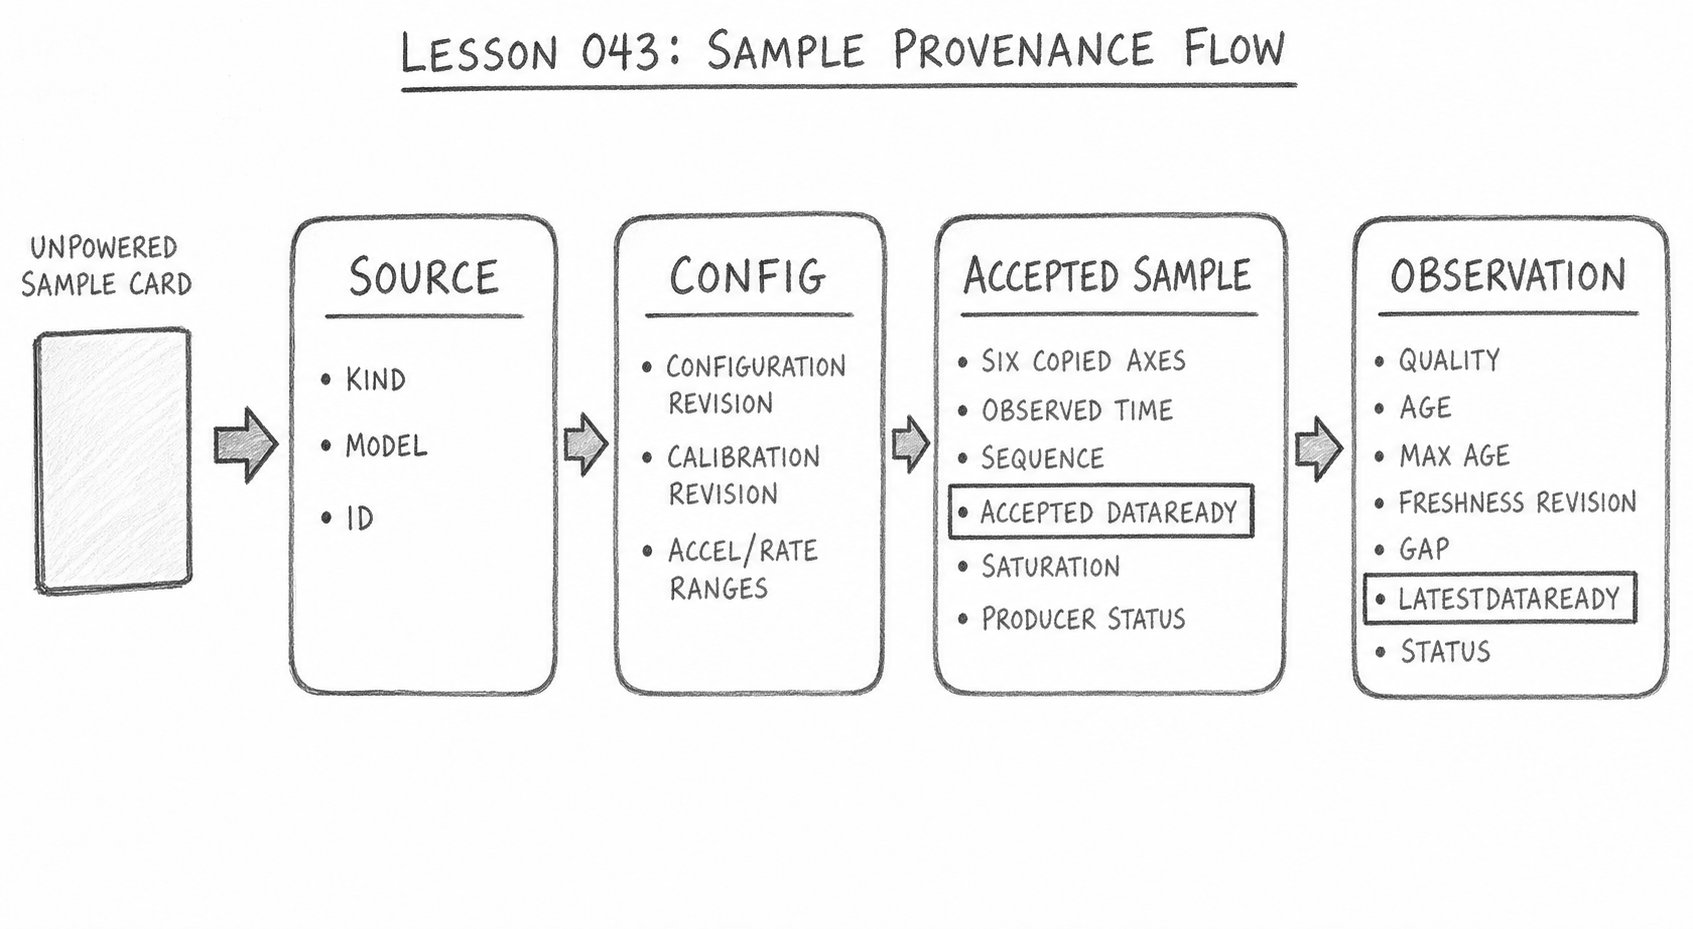
\includegraphics[width=0.96\linewidth,height=0.25\textheight,
 keepaspectratio]{043-inertial-provenance-pencil.png}

\small\textit{Alternative text: a pencil drawing follows a synthetic source
identity into one copied acceleration and angular-rate sample, then into
derived quality, age, and sequence-gap evidence without contacting hardware.}
\end{center}

The three acceleration fields use micro-g. The three angular-rate fields use
millidegrees per second. A vector gains its unit from the named field that
contains it; it is not a unit-free math type. \texttt{observedAt} and
\texttt{age} use milliseconds.

\begin{tabularx}{\linewidth}{@{}l X@{}}
\toprule
Evidence & Meaning\\
\midrule
source domain & kind, model, source ID, ranges, configuration and calibration revisions\\
accepted payload & timestamp, sequence, \texttt{sample.dataReady}, axes, saturation, and producer status\\
freshness contract & maximum age and its nonzero revision\\
latest evidence & \texttt{latestDataReady}, quality, age, gap, and status\\
\bottomrule
\end{tabularx}

Only the \texttt{SyntheticFixture}/\texttt{Synthetic} pair is accepted in E0.
The MPU6050 and QMI8658 names are negative-test seams, not supported adapters.

\newpage
\section{Predict the quality timeline}
\begin{center}
% ADK visual: pencil
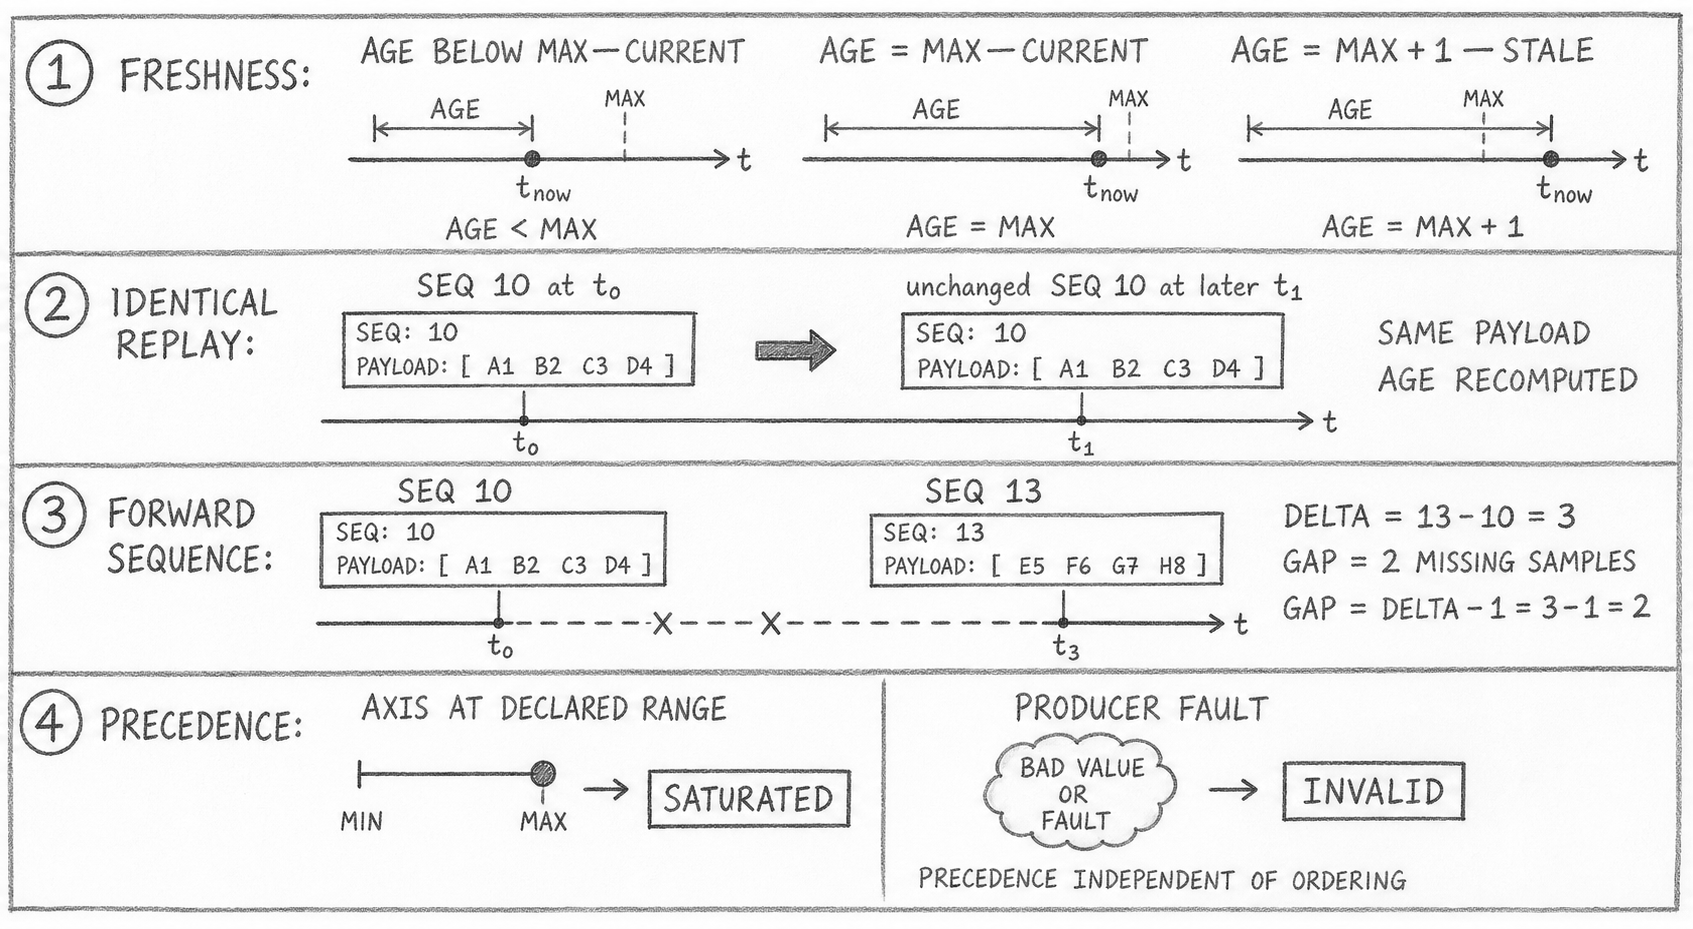
\includegraphics[width=0.97\linewidth,height=0.25\textheight,
 keepaspectratio]{043-inertial-timeline-pencil.png}

\small\textit{Alternative text: a pencil timeline shows an accepted synthetic
sample, an identical same-sequence replay aging from current to stale, a
separate saturated sample, and a producer fault; rejected evidence leaves the
last accepted sample unchanged.}
\end{center}

\begin{tabularx}{\linewidth}{@{}X X@{}}
\toprule
Condition & Predicted result\\
\midrule
age less than or equal to maximum & \texttt{Current}, status OK\\
age greater than maximum & \texttt{Stale}, status OK\\
same-sequence not-ready poll & retained ready payload; latest not ready; \texttt{Stale}\\
axis exactly at its declared range & \texttt{Saturated}, status OK\\
non-OK producer status & \texttt{Invalid}, producer failure retained\\
malformed identity, time, or value & \texttt{Invalid}, invalid argument\\
\bottomrule
\end{tabularx}

Precedence matters. Structural invalidity wins over staleness. Producer
failure makes numeric payload untrustworthy. For structurally valid payload,
saturation wins over age because bounded measurement meaning is already lost.

\section{Replay worksheet}
Use the constant frames in
\href{https://github.com/spincyc/adk/blob/main/examples/Lesson043InertialObservation/Lesson043InertialObservation.ino}
{the Lesson 043 replay sketch}. Before reading the result cells, complete the
prediction columns. Units belong in every numeric answer.

\begin{tabularx}{\linewidth}{@{}c l l X@{}}
\toprule
Frame & Prediction & Observed cell & Interpretation\\
\midrule
1 & quality: \blankline & \blankline & \blankline\\[5pt]
2 & gap: \blankline & \blankline & \blankline\\[5pt]
3 & ready/latest: \blankline & \blankline & \blankline\\[5pt]
4 & axes: \blankline & \blankline & \blankline\\[5pt]
5 & saturation: \blankline & \blankline & \blankline\\[5pt]
6 & age: \blankline ms & \blankline & \blankline\\[5pt]
7 & status: \blankline & \blankline & \blankline\\
\bottomrule
\end{tabularx}

The result cells are memory evidence for a host harness or simulator. The
sketch is compiled for packaging but is not run on a powered Mega in E0.
Serial output, a physical LED, and a debugger are not required or claimed.

\newpage
\section{Work the invariants}
\subsection*{Freshness calculation}
For wrap-safe forward time, calculate
\(\mathit{age}=\mathit{policyTime}-\mathit{observedAt}\).

\begin{tabularx}{\linewidth}{@{}X X X X@{}}
\toprule
policyTime (ms) & observedAt (ms) & maximumAge (ms) & quality\\
\midrule
\rule{0pt}{16pt}\blankline & \blankline & \blankline & \blankline\\[9pt]
\blankline & \blankline & \blankline & \blankline\\
\bottomrule
\end{tabularx}

At exactly \texttt{maximumAge}, predict \texttt{Current}. One millisecond
later, predict \texttt{Stale}. An exact semantic replay may make this
transition without creating a new sample or sequence gap.

\subsection*{Sequence calculation}
For a forward modular sequence delta \(d\), the recorded gap is \(d-1\).
Delta zero is accepted only when every named sample field is semantically
equal. The sole changed-field exception is a same-domain, same-sequence
\texttt{dataReady} true-to-false poll: it retains the accepted ready payload,
sets \texttt{latestDataReady} false, and publishes stale evidence. Delta
\texttt{0x80000000} is ambiguous and invalid. The poll creates no new sample,
sequence, or gap.

\begin{tabularx}{\linewidth}{@{}X X X X@{}}
\toprule
previous sequence & candidate sequence & predicted gap & accept/reject\\
\midrule
\rule{0pt}{16pt}\blankline & \blankline & \blankline & \blankline\\[9pt]
\blankline & \blankline & \blankline & \blankline\\[9pt]
\blankline & \blankline & \blankline & \blankline\\
\bottomrule
\end{tabularx}

\section{Diagnose without inventing evidence}
\begin{enumerate}
 \item Change one axis but retain the same sequence. Predict rejection. Verify
       that the previously accepted snapshot and history remain unchanged.
 \item Advance policy time while replaying the exact sample. Predict a later
       age and no new gap. Continue until quality becomes \texttt{Stale}.
 \item Change only \texttt{dataReady} from true to false at the same sequence.
       Predict retained axes and accepted readiness true, but latest readiness
       false and quality \texttt{Stale}.
 \item Place one axis exactly at its declared range and mark matching
       saturation. Predict \texttt{Saturated}; then remove the marker and
       predict structural rejection.
 \item Set \texttt{sourceId}, a revision, or a declared range to zero. Predict
       \texttt{Invalid}. Do not describe the result as a sensor reading.
 \item Supply \texttt{HardwareFailure}. Predict that producer failure
       dominates the numeric payload and that accepted history is preserved.
\end{enumerate}

\lessonbox{\textbf{Safe-state result.} This lesson acquires no hardware
resource, so reset clears policy history and returns the canonical invalid
snapshot. It cannot prove electrical shutdown, pin state, or power removal.}

\newpage
\small
\section{Separate acquisition from safe state}
\begin{tabularx}{\linewidth}{@{}>{\bfseries}l X X@{}}
\toprule
Stage & Predict & Observe and interpret\\
\midrule
Acquire & no endpoint; initialize valid config & status/result cells:
\blankline\\[10pt]
Observe & copy one bounded synthetic frame & quality/age/gap:
\blankline\\[10pt]
Reset & history clears; configuration remains & canonical snapshot:
\blankline\\
\bottomrule
\end{tabularx}

This separation is deliberate. Software initialization is resource-acquisition
evidence for a pure object. Reset is its software safe state. Neither is a
substitute for a future adapter's bus rollback or a module's electrical
inactive state.

\section{Malformed and deferred cases}
\begin{tabularx}{\linewidth}{@{}l X@{}}
\toprule
Case & Diagnosis\\
\midrule
stale & valid copied value exceeded its declared freshness window\\
not ready & same-sequence poll retains accepted ready payload; latest readiness is false; no new sequence or gap\\
saturated & valid copied axis reached its declared range; magnitude is bounded, not precise\\
unsteady & not classified here; Lesson 044 owns stationary-orientation eligibility\\
producer fault & source status is non-OK; numeric axes are not trusted\\
MPU/QMI source & unsupported in E0; exact specimen and adapter qualification remain open\\
\bottomrule
\end{tabularx}

\section{Blank E1 acceptance record}
\textbf{Do not prefill from compilation, replay, a datasheet, or this PDF.}

\begin{tabularx}{\linewidth}{@{}l X@{}}
\toprule
Required field & Bench record\\
\midrule
board revision / exact specimen & \blankline\\[7pt]
module and chip markings & \blankline\\[7pt]
supply / logic levels / instrument & \blankline\\[7pt]
tool version / tested commit & \blankline\\[7pt]
resource-acquisition prediction & \blankline\\[7pt]
resource-acquisition observation & \blankline\\[7pt]
safe-state prediction & \blankline\\[7pt]
safe-state observation & \blankline\\[7pt]
interpretation / reviewer / date & \blankline\\
\bottomrule
\end{tabularx}

\section{Evidence links}
\begin{itemize}
 \item \href{https://github.com/spincyc/adk/blob/main/src/inertial_observation.h}
       {Copied-observation public interface}
 \item \href{https://github.com/spincyc/adk/blob/main/tests/test_inertial_observation.cpp}
       {Deterministic Lesson 043 tests}
 \item \href{https://github.com/spincyc/adk/blob/main/examples/Lesson043InertialObservation/Lesson043InertialObservation.ino}
       {Compile-only synthetic replay}
 \item \href{https://github.com/spincyc/adk/blob/main/docs/design/LESSONS_043_045_BALANCE_TABLE_PLAN.md}
       {Lessons 043--045 design and open gates}
\end{itemize}

The searchable HTML lesson is the hardware-independent accessible route.
This untagged print edition makes no PDF/UA, powered-module, or physical
acceptance claim.
\end{document}
